\specialchap{序言}

随着物理学的发展,人们对于这个世界的理解也越来越深入。在粒子物理的相关研究中,组成世界的基本粒子一共有12种,分为6种夸克,3种带电轻子以及三种中微子。随着对于这十二种粒子的深入研究和理解,人们在量子场论的框架下构建了基于量子色动力学和弱点相互统一理论的标准模型(Standard Model, SM)。标准模型成功的解释了宇宙中物质的构成以及他们之间的相互作用,并被大量的实验所证明。尤其是2012年标准模型所预测的最后一种粒子——希格斯玻色子被发现,更是完美的符合了标准模型的预测。

在标准模型所描述的基本粒子中,中微子是其中性质十分的特殊,也是最神秘的一个。对中微子的研究最早可以追溯到1930年,奥地利物理学家泡利(Wolfgang Ernst Pauli)在一封解释$\beta$衰变问题的信中,提出了一种微小的电中性粒子以解释衰变中能谱连续的问题。这个假设被费米(Enrico Fermi)引入到了他的$\beta$衰变理论中\supercite{wilson1968fermi}。而后在
1956年,Clyde Cowan和Frederick Reines首次确认了电子中微子的存在\supercite{cowan1991detection},于是中微子揭开了它隐藏的面纱,被人们所渐渐了解。$\mu$中微子于1962年被Brookhaven国家实验室所发现\supercite{danby1962observation},而后知道2000年,最后一种中微子$\tau$中微子存在的直接证据才被费米实验室所找到\supercite{kodama2001observation}。

标准模型中中微子被认为是没有质量的,然而过往和正在进行的大量中微子实验,如超级神冈(Super-Kamiokande)\supercite{fukuda1998evidence},萨德伯里中微子观测站(SNO)\supercite{ahmad2002direct}等,都观测到了中微子震荡现象。对这些现象最为自然的解释就是中微子是有质量的,这也可能标志着标准模型之外的,未被探索的新物理。

中微子既然可能有质量,那么它质量的来源便是一个十分有趣的问题。如果假设中微子是狄拉克费米子(Dirac fermions),那么为了使中微子产生质量,中微子与希格斯场相互作用的耦合系数会比夸克等粒子小12个量级,这种模型解释起来会变得十分的困难。另一种假设是中微子是马约拉纳费米子(Majorana fermions),即中微子自身是自己的反粒子,这种模型相对而言更为自然自洽,但它也意味着标准模型中的轻子数守恒的推断将会被打破,这将会对理论物理带来巨大的改变。然而到现在为止,还没有足够的实验观测能够判断哪种模型更为正确。

在中微子到底是哪种费米字的相关研究中,有一类实验是在寻找被称作无中微子双Beta衰变(Neutrinoless double beta decay, NLDBD)\supercite{avignone2008double}的稀有事件。在标准模型中,有一些核素不能直接进行普通的Beta衰变,但是他们可以通过一个次级的弱相互作用来同时释放出两个电子(正电子)和两个反中微子(中微子),这种衰变模式被称作双Beta衰变(Double beta decay, DBD),如图\ref{fig:nldbd}(a)所示,这种衰变过程也已经被实验所观测到了。如果中微子是马约拉纳费米子,这就意味着中微子和反中微子完全一致,那么双Beta衰变中第一次释放出的反中微子(中微子)又可能作为中微子(反中微子)参与了第二次衰变,即直接衰变出两个电子(正电子)而不产生反中微子(中微子),如图\ref{fig:nldbd}(b)所示。这种现象就被称作无中微子双Beta衰变(后称NLDBD)事件。

\begin{figure}
    \centering
    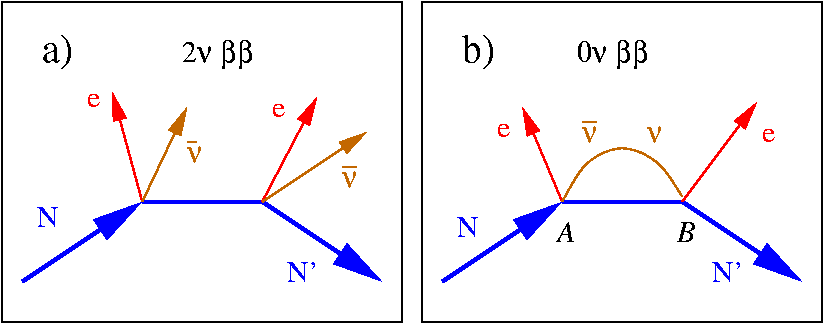
\includegraphics[width=0.5\columnwidth]{pic/nldbd.png}
    \caption{有中微子双Beta衰变(a)以及无中微子双Beta衰变(b)示意图。}
    \label{fig:nldbd}
\end{figure}

如果NLDBD事件被探测发现,那么不单单意味着轻子数不再守恒,中微子的质量也可以通过NLDBD事件的发生概率计算得到,如公式\ref{eq1}所示\supercite{avignone2008double}。其中$G^{0\nu}$是相空间因子,$M^{0\nu}$是核矩阵元素。如果能够测量得到NLDBD事件的半衰期,那么马约拉纳中微子质量$\langle m_{\beta\beta}\rangle$就可以计算得到,进而可以得到中微子绝对质量量级和中微子的质量顺序,使得人们对中微子能够获得进一步的认识。

\begin{equation}
    (T_{1/2}^{0\nu})^{-1}=G^{0\nu}|M^{0\nu}|^2\frac{\langle m_{\beta\beta}\rangle ^2}{m_e^2}
    \label{eq1}
\end{equation}

这些年来世界上很多实验组都在探测无中微子双Beta衰变,根据2015年美国核科学顾问局的报告\supercite{NLDBD_NSAC},现在正在进行的实验包括CUORE\supercite{Artusa:2014lgv},EXO-200\supercite{Albert:2014awa},GERDA\supercite{Agostini:2016iid},
KamLAND-Zen\supercite{KamLAND-Zen:2016pfg},
Majorana\supercite{Abgrall:2013rze},SNO+\supercite{Andringa:2015tza}等,最好的实验结果是KamLAND-Zen
给出的关于$^{136}$Xe的无中微子双Beta
衰变,其半衰期大于$1.07\times10^{26}$年。现在世界上的NLDBD
实验组普遍达成了共识,至少需要1吨级别的放射性同位素才有可能通过探测NLDBD
事件确定中微子的质量顺序。为了顺利的完成这一量级的实验,需要能够顺利的生产出吨级的同位素,同时需要极佳的探测器分辨率和极低的本底噪声,以及鉴别NLDBD
和本底的方法。

粒子和天气物理氙探测器第三期实验(Particle And Astrophysical Xenon Experiment III,以下简称PandaXIII)便是一个设计中的吨级的$^{136}$Xe无中微子双Beta衰变探测实验,它使用高压气氙时间漂移室(TPC)作为探测器,放置于锦屏地下实验室来屏蔽宇宙射线本底,并计划在两到三年内建立出第一个200kg级探测器。本文详细描述了PandaXIII实验设计和前期测试中模拟的相关工作,分为以下几个部分。第一章将会简单介绍整个项目,第二章描述了探测器模拟中本底模拟的相关工作,第三章介绍了如何使用卷积神经网络(Convolution Neural Network, CNN)来鉴别本底事件和信号,第四章给出了原型探测器测试标定过程中的模拟工作。上述工作是本文作者主要参与的,PandaXIII项目中探测器设计,电子学等其他相关工作的描述可以参见PandaXIII中期设计报告\supercite{cdr}。

% vim:ts=4:sw=4